\chapter{O modelo de estimação do juros da dívida técnica}
\label{estimacao:juros}

Neste capítulo definiremos um modelo para estimação dos juros da dívida técnica baseado na variação da produtividade nos projetos de desenvolvimento de software. Inicialmente, iremos descrever a versão de alto nível desse modelo e em quais ideias ele está baseado. Em seguida, forneceremos uma descrição de uma aplicação desse modelo na estimação dos juros da dívida técnica em projetos de software livre.



\section{Introdução}



Tradicionalmente, os juros da dívida técnica são definidos como o conjunto das dificuldades adicionais, causadas pela existência da dívida, para realizar as atividades de desenvolvimento de software. Caso a dívida técnica não estivesse presente, essas dificuldades não existiriam. Nesta pesquisa, sugerimos uma nova perspectiva para analisar os juros da dívida técnica e, assim, permitir seu gerenciamento: considerá-los como a causa de uma diminuição da produtividade dos projetos. 

Quanto mais juros um projeto tem, menor a produtividade real, quando comparada à obtida em um cenário onde não houvesse dívida técnica. Essa redução acontece, pois mais recursos terão de ser utilizados para se atingirem os mesmos objetivos. Vamos ilustrar essa  degradação na produtividade com um exemplo: 

\begin{tcolorbox}
Uma empresa de desenvolvimento de software resolve iniciar um projeto para o desenvolvimento de algumas novas funcionalidades para um sistema de vendas existente. Ao realizar uma análise de viabilidade, o time responsável descobre que o código atual do sistema apresenta uma documentação insuficiente, problemas de arquitetura e design e quantidade de testes unitários não compatível com o nível de qualidade esperado para o projeto. O time conclui, corretamente, que haverá uma série de dificuldades adicionais para a conclusão do projeto. 
\end{tcolorbox}

Nesse exemplo, fica claro que a produtividade do time seria melhor caso esses problemas identificados não existissem. Ou seja, menos recursos teriam de ser gastos para alcançar os mesmos objetivos. Os problemas encontrados são as dívidas técnicas do software que foram sendo adquiridas com o passar do tempo. As dificuldades para se realizar o projeto de adição das funcionalidades adicionais são os juros causados por essas dívidas. Observando o exemplo fornecido, proporemos um modelo, no qual a estimativa dos juros da dívida técnica será calculado como a diferença de produtividade entre dois cenários: um com dívida técnica, semelhantemente ao exemplo fornecido, e um cenário onde essas dívidas técnicas não existam. Como discutiremos mais à frente, na verdade, o cenário onde não existe dívida é inalcançável. O que usaremos será uma aproximação em que a dívida técnica seja muito baixa. 


\section{Avaliação da produtividade dos projetos de software}
\label{modelo_de_estimacao_produtividade}

O termo produtividade é usado para descrever a proporção entre o valor dos recursos utilizados em um processo e o valor do que é efetivamente produzido. Os recursos aplicados são chamados de entradas, enquanto os resultados do processo são chamados de saídas. O problema de medir a produtividade de um processo pode ser resumido em duas partes:

\begin{enumerate}
\item Identificar as entradas e as saídas.
\item Quantificar  as entradas e saídas de tal forma que a relação entre elas possa ser calculada
\end{enumerate} 

O processo mais eficiente é aquele no qual mais valor (saídas) é produzido utilizando menos recursos (entradas).

Existe uma série de desafios para identificar e quantificar as entradas e saídas do processo de desenvolvimento de software. Devido à inerente complexidade desse processo, existem diversas possibilidades para quais serão as entradas e saídas a serem incluídas na análise de produtividade. A quantidade de homens/hora e a quantidade de linhas de código produzidas são métricas normalmente utilizadas como entrada e saída respectivamente.  Entretanto, essas métricas, apesar de poderem ser consistentemente medidas, são demasiadamente imprecisas, já que existem diversos outros fatores relevantes conforme mostrado no estudo de MacCormack et al. \cite{maccormack2003trade}. No caso da quantidade de homens/hora, por exemplo, um outro fator importante é o nível de experiência das pessoas envolvidas. A hora de um colaborador inexperiente naturalmente será menos valiosa do que a hora de um com mais experiência. Semelhantemente, a quantidade de linhas de código produzidas, apesar de muito utilizada, também é uma métrica imprecisa já que não inclui uma quantificação do valor dessas linhas de código.  É possível que uma grande quantidade de linhas de código seja criada para realizar uma atividade, porém, essa mesma atividade possa ser desenvolvimento com uma quantidade bem menor. Além desses dois exemplos, existem outras entradas e saídas que podem ser utilizadas em modelos de medição de produtividade conforme mostrado por Hernández-López et al.,\cite{hernandez2015productivity}. Podemos observar que não existe uma forma totalmente precisa para se avaliar a produtividade dos processos de desenvolvimento de software. Isso se dá não apenas pela existência de diversas medidas possíveis como também devido aos aspectos subjetivos dessas medidas. 

\subsection{Modelos baseados em expectativa de produção}

Para medir a produtividade no nosso modelo de estimação, utilizamos uma proposta de Kitchenham e Mendes \cite{kitchenham2004software}. Nesse trabalho os autores sugerem um modelo onde a produtividade de um processo de desenvolvimento de software é avaliada comparando o esforço estimado para a realização de um determinado projeto com o esforço efetivamente gasto. Essa relação é representada pela equação ~\ref{eq:model}. O esforço estimado, representado pela variável \textit{AdjustedSize}, é calculado por meio de uma regressão linear múltipla utilizando dados históricos de projetos similares. A variável $Effort$ é o esforço efetivamente gasto para a realização do projeto. Se a variável $Productivity$ for maior que 1 quer dizer que o projeto foi realizado com menos esforço do que o esperado levando-se em consideração os dados dos projetos semelhantes.
 
 
 

\begin{equation}
\label{eq:model}
  Productivity = AdjustedSize/Effort
\end{equation}


O modelo descrito na equação \ref{eq:model} não determina quais medidas serão utilizadas para quantificar as variáveis $AdjustedSize$ e $Effort$. Isso é esperado já que essas medidas são diferentes para cada domínio da aplicação sendo desenvolvida. Os autores fornecem um exemplo da aplicação do modelo em um projeto de desenvolvimento web. Nesse exemplo, são utilizados o número de páginas, o número de imagens e o número de funcionalidades da aplicação como medidas para estimar o esforço. 

Apesar da viabilidade dessa estratégia, os autores  concluem que calcular a produtividade esperada, utilizando os  fatores associados, é uma atividade complexa e que também não pode ser feita com precisão absoluta \cite{petersen2011measuring}.

Devido à importância, nesta pesquisa, do modelo de produtividade representado pela equação \ref{eq:model}, forneceremos um exemplo de como ele deve ser utilizado. Na Tabela \ref{tab:examplo_aplicacao_modelo_produtividade} há a quantidade de linhas produzidas e a quantidade de desenvolvedores de três projetos fictícios. Podemos estimar, utilizando os dados desses três projetos, qual seria a quantidade de desenvolvedores necessários para produzir a quantidade de linhas de código do projeto. Essa estimação é realizada por meio de uma regressão linear\cite{degroot2012probability} tendo como variável explicativa o número de linhas de código e como variável explicada o número de desenvolvedores. Realizando essa regressão linear, podemos calcular os valores ajustados para o número de desenvolvedores.

No exemplo da Tabela \ref{tab:examplo_aplicacao_modelo_produtividade}, podemos observar que o projeto A envolveu cinco desenvolvedores, porém, o número esperado, tendo como base os dados dos outros projetos, seria 5,33.  portanto, o projeto A conseguiu produzir 15.000 linhas de código com uma quantidade menor do que  a esperada de desenvolvedores. A razão entre a quantidade esperada e a quantidade real de desenvolvedores é a produtividade do projeto, de acordo com a equação \ref{eq:model}. Por outro lado, o projeto B tem uma quantidade de desenvolvedores maior do que a esperada. Com isso, a produtividade desse projeto foi menor do que 1, o que o leva a ser considerado um projeto menos produtivo do que o projeto A.

\begin{table}[H]
\centering
\begin{tabular}{lllll}
\hline
\textbf{Projeto} & \textbf{Linhas de código} & \textbf{Nº Desen.} & \textbf{Nº  Desen. ajustado}  & \textbf{Produtividade}\\ \hline
A                & 15.000                     & 5       & 5.33  &        1,06          \\ \hline
B                & 20.000                     & 8       & 7.33   &       0,91         \\ \hline
C                & 25.000                     & 9        & 9.33    &      1,03         \\ \hline
\end{tabular}
\caption{Quantidade de linhas de código, número de desenvolvedores, número de desenvolvedores ajustado e produtividade de três projetos de software fictícios.}
\label{tab:examplo_aplicacao_modelo_produtividade}
\end{table}





\section{O modelo de estimação dos juros da dívida técnica}
\label{modelo_abstrato}


A sustentação lógica do nosso modelo de estimação dos juros é baseada na existência de dois cenários nos quais um mesmo projeto de software pode ser desenvolvido:

\begin{itemize} 
\item  \textbf{sem dívida técnica}. Nesse cenário, a produtividade de um projeto de software é a melhor possível com os recursos disponíveis, ou seja, levando-se em consideração todo o contexto no qual o projeto é desenvolvido, a produtividade obtida é a melhor que poderia ser alcançada. 
\item \textbf{com dívida técnica}. Esse cenário é idêntico ao cenário \textbf{sem dívida técnica}, exceto por uma diferença: existem dívidas técnicas.   Todas as outras variáveis relacionadas com o contexto do projeto são exatamente as mesmas. Ou seja, as atividades a serem realizadas são as mesmas e com o mesmo nível de complexidade.
\end{itemize}

  

É importante notar que o cenário totalmente sem dívida técnica nunca existirá já que não é possível a existência de um software sem nenhuma dívida técnica. Temos algumas razões para afirmar a inexistência de projetos sem nenhuma dívida técnica. A primeira delas é o fato de que a própria identificação do que é ou não uma dívida técnica é subjetiva e muitas vezes intangível. A segunda razão é associada às dívidas técnicas de tecnologia. Com o passar do tempo uma tecnologia vai se tornando obsoleta e continuar a utilizá-la pode trazer esforços adicionais. Com isso, devido à contínua criação de novas tecnologias, é impossível garantir que não haja algum tipo de obsolescência. 


Vamos revisitar agora o exemplo anteriormente fornecido neste capítulo incluindo as definições dos dois cenários de desenvolvimento e outros conceitos já introduzidos: 

\begin{tcolorbox}

Um determinado projeto de desenvolvimento que consistia em adicionar um conjunto de novas funcionalidades a um sistema já existente foi realizado em um cenário \textbf{com dívida técnica}. Ou seja, esse sistema existente possuía um número  $D$ de dívidas técnicas.  Esse projeto adicionou uma quantidade $S$ de funcionalidades ao sistema. Para obter o resultado  $S$  foi utilizada  uma equipe de desenvolvimento de software de tamanho $E$ obtendo uma produtividade $Y$.   Com isso, a produtividade $Y$ do projeto pode ser calculada de acordo com a equação \ref{eq:juros_1}. Por meio da equação \ref{eq:juros_1}, representamos a degradação da produtividade causada pela existência da dívida técnica $D$. Quanto maior $D$, menor será a produtividade do projeto.

\begin{equation}
\label{eq:juros_1}
Y =  \frac{S}{D*E}
\end{equation}

\end{tcolorbox}




Imagine que seja possível que esse mesmo projeto pudesse ser realizado novamente pela mesma equipe e em um contexto exatamente igual, porém sem que a equipe pudesse lembrar da primeira execução e usar o que aprendeu nela. Além disso, nesta segunda execução, a dívida técnica do projeto não existe. Ou seja, o projeto dessa vez foi realizado em um cenário de \textbf{sem dívida técnica}. Logo, a produtividade do time de desenvolvimento será outra que chamaremos de $\overline{Y}$. A produtividade  $\overline{Y}$ pode ser calculada utilizando a Equação \ref{eq:juros_2}. 

É evidente que  a produtividade $\overline{Y}$ será melhor do que a produtividade  $Y$ já que a única diferença entre os dois cenários, nesse exemplo fictício,  é a existência ou não de dívida técnica. Sem a dívida técnica, o time terá mais facilidade para desenvolver as funcionalidades do projeto e com isso elas serão desenvolvidas em um menor tempo aumentando, assim, a produtividade. Observando esse exemplo fictício podemos inferir a Equação \ref{eq:juros_3} em que $J$ é os juros da dívida técnica que foi pago durante a execução do projeto de desenvolvimento no cenário de \textbf{produtividade afetada}. \textit{\textbf{Note que, para este exemplo fictício,  $J$ não  é uma estimativa dos juros, ao invés disso, é um valor exato}}.  

Esse exemplo fictício obviamente não pode ser reproduzido exatamente como descrito. Um motivo é a impossibilidade de executar o mesmo projeto duas vezes com o mesmo time sem que a segunda execução seja facilitada pelas experiências obtidas pela primeira. Outro motivo é a impossibilidade de se remover totalmente a dívida técnica $D$ do sistema existente. Contudo, esse exemplo apresenta-se útil como uma argumentação lógica para uma estratégia onde possa ser encontrado um valor aproximado para $J$ em situações reais.

\begin{equation}
\label{eq:juros_2}
\overline{Y} =  \frac{S}{E}
\end{equation}


\begin{equation}
\label{eq:juros_3}
J = \overline{Y} - Y
\end{equation}

\subsection{Estimação dos juros por aproximação}
\label{estimacao_juros_por_aproximacao}

Conforme descrito anteriormente, não podemos calcular precisamente os juros da dívida técnica utilizando a Equação \ref{eq:juros_3}. Porém, utilizaremos essa fórmula e a situação fictícia que descrevemos como uma base lógica para o cálculo de uma estimativa dos juros da dívida técnica. Para isso, precisamos de valores estimados para $Y$ e $\overline{Y}$. Nossa estratégia será a de estimar o valor de $Y$ utilizando os projetos no cenário  \textbf{com dívida técnica} e o valor de $\overline{Y}$ utilizando os projetos no cenário  \textbf{sem dívida técnica} da seguinte forma:

\begin{enumerate}
\item Selecionamos um projeto A que tenha um nível normal de dívida técnica.  A produtividade desse projeto será a variável $Y$ da equação  \ref{eq:juros_3}.
\item Selecionamos um projeto B  que seja muito semelhante ao projeto A, porém tenha um nível de dívida técnica muito baixo, ou seja, esteja no cenário  \textbf{sem dívida técnica}. A produtividade desse projeto será a variável $
\overline{Y}$ da equação  \ref{eq:juros_3}. O limite de dívida técnica  que um projeto pode ter e ainda ser considerado pertencente a esse cenário dependerá do contexto desse projeto. 
\item Calculamos um valor estimado para $J$ usando a equação \ref{eq:juros_3}.
\end{enumerate}

Com isso, estamos simulando a remoção da dívida $D$ do projeto A e criando uma aproximação da realização do projeto A sem a existência de dívida técnica, o que nos permite a estimação do valor de $J$, que representa os juros da dívida técnica do projeto A.

Como veremos no nosso estudo de caso do Capítulo \ref{cap_estudo_caso}, podemos usar mais de um projeto para representar as variáveis $Y$  e  $\overline{Y}$ da seguinte forma:

\begin{enumerate}
\item Definimos um grupo $G$ de projetos que sejam todos semelhantes entre si.
\item Dividimos o grupo $G$ em duas partições: 
\begin{enumerate}
\item[$P_1$] Projeto no cenário \textbf{sem dívida}
\item[$P_2$] Projetos no cenário \textbf{com dívida}.
\end{enumerate}
\item Atribuímos a produtividade média dos projetos na partição $P_1$ à variável $\overline{Y}$.
\item Atribuímos a produtividade média dos projetos na partição $P_2$ à variável $Y$.
\item Calculamos um valor médio para $J$ usando a equação \ref{eq:juros_3}. Nesse caso, $J$ representa a média de juros da dívida técnica dos projetos na partição $P_2$
\end{enumerate}
 
 \subsection{Abstração do modelo}
 
Nosso modelo de estimação dos juros é um modelo abstrato.  Não há uma definição de quais métricas serão utilizadas tanto para a estimação da dúvida quanto para a estimação da produtividade.  Para que esse modelo possa ser aplicado, é necessário que exista uma definição precisa a respeito de quais métricas serão utilizadas para avaliar a produtividade e qual processo será realizado para estimar os juros da dívida técnica.  Entretanto essas definições dependem das características dos projetos avaliados. Por exemplo, o conjunto de dívidas técnicas em um projeto no qual o paradigma de desenvolvimento seja o orientado a objetos é diferente do conjunto de dívidas técnicas de um projeto que utilize o paradigma funcional. Por isso, essas definições, nessárias para aplicação do modelo proposto, precisam ser feitas de acordo com o contexto. Ou seja, para aplicar o modelo, é necessário criar uma instância dele conforme ilustrado na Figura \ref{fig:cap_metodo_niveis_abstracao}.


  \begin{figure}[H]
  \centering
  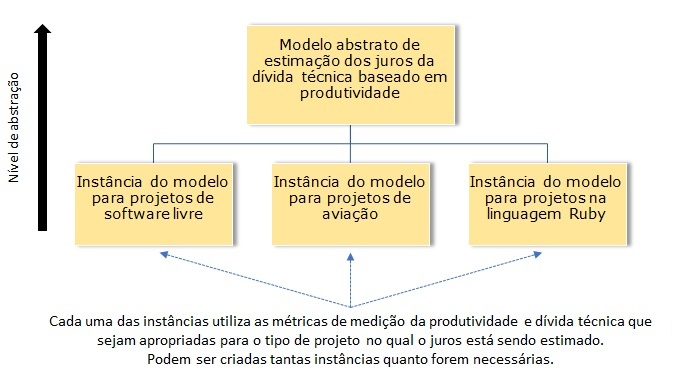
\includegraphics{capitulo_metodo/NiveisDeAbstracoesModelo.jpg} 
  \caption{Níveis de abstração do modelo de estimação dos juros da dívida técnica. }
  \label{fig:cap_metodo_niveis_abstracao} 
\end{figure}


 
 \section{Criação das instâncias do modelo de estimação dos juros da dívida técnica}
  
Para instanciar o modelo de estimação é necessário definir certas métricas que serão utilizadas para avaliar a produtividade dos projetos. Além disso, será necessário definir como agrupar os projetos semelhantes como também particionar cada um desses grupos de forma a separar os projetos nos cenários \textbf{com dívida técnica} e \textbf{sem dívida técnica}. A tabela \ref{cap_modelo_tabela_resumo_passos} resume todas as definições que precisam ser feitas para a instanciação do modelo para a estimação dos juros da dívida técnica.  A seguir descreveremos cada uma dessas atividades.
 
 
 \begin{table}[H]
 \centering
\caption{Atividades necessárias para a criação de um modelo concreto de estimação dos juros da dívida técnica específico.}
\label{cap_modelo_tabela_resumo_passos}
\begin{tabular}{l|l}
\hline
 & \multicolumn{1}{c}{Atividade}                                \\ \hline
1  & Seleção das métricas que representam as entradas do processo  \\ \hline
2  & Seleção das métricas que representam as saídas do processo    \\ \hline
3  & Definição do método de agrupamento dos projetos semelhantes   \\ \hline
4  & Definição do método de particionamento dos grupos de projetos \\ \hline
\end{tabular}
\end{table}


\subsection{Seleção das métricas que representam as entradas do processo}

Em um modelo de avaliação de produtividade de um processo, as entradas representem aquilo que é gasto para que o resultado do processo seja alcançado. Nessa etapa, são definidas quais entradas serão utilizadas. Na avaliação da produtividade em projetos de software, normalmente são usadas como entradas métricas relacionadas ao esforço necessário para a produção do software. Esse esforço é medido tradicionalmente por meio da quantidade de pessoas que foram alocadas para o projeto e pela quantidade de tempo na qual essas pessoas atuaram. Entretanto, existe uma série de aspectos que pode afetar a medida de esforço em uma análise de produtividade e que pode ser incluída nos modelos específicos para torná-los mais precisos. A literatura nos fornece alguns desses aspectos conforme listaremos a seguir:

\begin{itemize}

\item O nível de experiência  da equipe tem uma influência direta na avaliação de produtividade de um projeto de software.  Um exemplo em que isso pôde ser verificado empiricamente pode ser encontrado no trabalho de Kitchenham et al.\cite{kitchenham2004software}. Um dos resultados dessa pesquisa mostrou uma divergência significativa entre o nível de produtividade medido pelo modelo sugerido pelos autores e a produtividade medida pela empresa para um projeto real. A produtividade medida pelo modelo foi muito baixa, porém, a empresa considerava que o projeto foi  extremamente bem sucedido. Ao analisar com detalhes os dados obtidos, os pesquisadores concluíram que o projeto foi realizado por uma equipe júnior e inexperiente. Contudo, ele foi realizado em um tempo satisfatório pela empresa. Como o modelo da pesquisa não utilizava informações a respeito da experiência dos profissionais, o modelo não foi capaz de identificar que se trata,  sim, de um projeto produtivo, pois foi realizado com uma equipe menos experiente e consequentemente mais barata. 
Além do tempo, o fator conhecimento também pode ser incluído em um modelo de análise de esforço. Um profissional pode trabalhar por muito tempo em uma determinada atividade sem que ele realmente adquira novos conhecimentos e melhore a execução das suas responsabilidades. Por outro lado, um profissional com menos tempo pode se dedicar ao seu crescimento individual e alcançar resultados melhores do que o de profissionais com mais anos de experiência. Isso se torna especialmente importante no contexto da análise de produtividade quando a organização investe no aperfeiçoamento individual. Os custos desse desenvolvimento podem ser incorporados como esforço no modelo de análise de produtividade.
\item O tempo gasto pela equipe de desenvolvimento não é exclusivamente gasto produzindo código. De acordo com Wagner et al. \cite{wagner2018systematic}, até um terço do tempo de um  desenvolvedor é  usado com reuniões, apresentações, gestão de projetos e realização de cursos para o aprimoramento individual. Se no contexto no qual o software está sendo desenvolvimento há uma priorização para atividades não técnicas como essas, é possível que o resultado da análise de produtividade seja prejudicado. Essa questão se torna especialmente preocupante quando o objetivo é avaliar a produtividade de projetos em contextos diferentes. Um projeto em um ambiente muito burocrático, por exemplo, no qual sejam realizadas muitas reuniões que não estejam relacionadas ao projeto, pode ser considerado como improdutivo caso o tempo gasto com essas reuniões seja contabilizado como tempo gasto no projeto.

\item Alguns fatores não técnicos podem influenciar a produtividade de uma equipe. De acordo com uma revisão sistemática realizada por Wagner et al. \cite{wagner2018systematic}, esses fatores são relacionados à aspectos como o quão amigável é o ambiente no qual o software é desenvolvido, a diferença de temperamentos entre os membros do time de desenvolvimento e a adequação do local de trabalho para a realização de atividades que exijam criatividade.


\end{itemize}


Apesar de essas informações aparentemente adicionarem maior precisão aos modelos de produtividade, nem sempre elas poderão ser utilizadas. O primeiro motivo é a possível inexistência de dados que tornem possível a sua medição. Por exemplo, muitos repositórios de software não possuem informações detalhadas a respeito do histórico dos seus membros. Isso inviabiliza medir o nível de experiência de um determinado contribuidor. Além disso, algumas das informações que poderiam incrementar a precisão das métricas de esforço são difíceis de serem medidas. Um exemplo é o nível  adequação do local de trabalho  para a realização de trabalho criativo. Para obterem-se dados para medir esses aspectos podem ser realizadas entrevistas ou utilizados questionários. Entretanto essa medição pode-se tornar cara quando o número de colaboradores e projetos é muito grande. Além disso, vale reforçar, dificilmente essas informações são encontradas em repositórios públicos com informações sobre projetos de software.

\subsection{Seleção das métricas que representam as saídas do processo}
\label{modelo_concreto_saidas}

Há uma dificuldade adicional na escolha das métricas de saída em um modelo de avaliação da produtividade em projetos de software. Essa dificuldade é causada pelo fato de que normalmente as reais saídas de um projeto são subjetivas. Apesar de o número de linhas de código serem utilizadas extensivamente, essa métrica pode dizer muito pouco a respeito do valor que realmente foi produzido durante o projeto. Um projeto pode ter uma quantidade alta de linhas de código e, ainda assim, não atingir seus objetivos. Com isso, uma métrica que considere os objetivos do projeto de software pode ser mais adequada para medir o que foi produzido. Uma das alternativas é a utilização dos pontos por função. Nessa técnica de medição é estabelecida, pelo usuário do software, uma pontuação para cada funcionalidade. Essa pontuação é independente da tecnologia ou linguagem que será utilizada para implementar a funcionalidade. O tamanho do software é, então, medido pela quantidade total de pontos de todas as suas funcionalidades\cite{jeffery1997function}. Apesar de a quantidade de linhas de código e de os pontos por função serem utilizados largamente como métricas para representar o tamanho do software, aquelas sozinhas podem não ser suficientes para capturar todos os aspectos necessários para realmente calcular o tamanho de um projeto. 

Cada contexto pode exigir métricas diversas para capturar os objetivos do projeto e consequentemente seu tamanho. Um exemplo fornecido por Kitchenham et al.\cite{kitchenham2004software} é de projetos de websites. A quantidade de linhas de código ou os pontos por função podem ser adequados para medir o tamanho das funcionalidades dinâmicas do website tais como comércio eletrônico e  interação dos usuários com o conteúdo. Entretanto, algumas características estáticas como as imagens e o número de páginas com conteúdo estão diretamente ligadas ao esforço necessário para realizar o projeto e, ainda assim, não podem ser capturadas por essas duas métricas. Outro exemplo são os projetos de software livre.  Nesses projetos, os objetivos a serem alcançados também são as funcionalidades que serão disponibilizadas aos seus usuários. Porém, no contexto desses projetos, pode ser adequado incluir outras métricas como popularidade e facilidade de colaboração para representar o tamanho do software. 

De acordo com Kitchenham et al.\cite{kitchenham2004software}, em um modelo de análise de produtividade, é necessário que as métricas utilizadas para representar as saídas do processo de desenvolvimento estejam relacionadas com as métricas utilizadas para representar o esforço. Isso quer dizer que, estatisticamente, deve haver uma correlação não nula entre o esforço e cada uma dessas métricas de tamanho. Ou seja, a medida que mais ou menos esforço seja realizado, deverá haver um impacto no valor das variáveis de tamanho. Essa correlação se explica pelo fato de que seria incoerente incluir em uma análise de produtividade informações que não são afetadas pelo valor gasto para produzir as saídas. Isso acontece, pois uma medida de produtividade é, por definição, a relação entre o quanto se gasta e o quanto se produz. 







\subsection{Definição do método de agrupamento dos projetos semelhantes }

Conforme descrito na seção \ref{modelo_abstrato}, nosso modelo abstrato de estimação dos juros da dívida técnica é baseado na ideia de que os juros são as dificuldades adicionais para desenvolver o software e que essas dificuldades não seriam encontradas caso não houvesse a dívida técnica. Os juros podem ser calculados como a diferença de produtividade em um cenário com a dívida técnica e um cenário sem a dívida técnica. Conforme explicado na seção \ref{modelo_abstrato}, a criação desses cenários é inviável. Contudo, propomos, ao invés do cálculo exato, uma estimação dos juros por meio de uma aproximação. Essa estimação é obtida ao compararmos a produtividade de projetos semelhantes, de modo que, uma parte desses projetos possui um nível pequeno de dívida técnica enquanto a outra parte possui um nível normal ou grande.  Para se realizar essa comparação, precisamos identificar se um projeto é semelhante a outro. O modelo abstrato descrito na seção \ref{modelo_abstrato} não define como essa análise de similaridade deve ser realizada. Seria difícil descrever uma estratégia de análise de similaridade que possa ser utilizada em todas as situações. Por isso, a estratégia que será utilizada deve ser definida em cada um dos modelos concretos de estimação dos juros da dívida técnica.


Na literatura podem ser encontradas algumas abordagens para a análise de similaridade entre projetos de software:
 
\begin{enumerate} 
\item  Barreto et al.\cite{barreto2010analyzing}, calculam a similaridade entre projetos usando cinco características: objetivo do projeto, medida usada para indicar os objetivos do projeto, cliente, experiência do time de desenvolvimento e experiência do gerente de projetos.  Para calcular uma medida numérica é fornecido um modelo matemático no qual a similaridade entre dois projetos é calculada pelo somatório do inverso da diferença entre cada uma das características do projeto. Cada uma das características tem um peso calculado de acordo com a relevância indicada pelos especialistas. Uma das limitações desse trabalho é a de que ele considera apenas características numéricas dos projetos ou converte as características não numéricas em numéricas. Porém, algumas características de um projeto de software podem ser medidas por meio de variáveis categóricas. As variáveis categóricas representam informações qualitativas do projeto. Um exemplo seria a variável complexidade. Ela pode possuir valores como baixa, média ou alta. 

\item Uma abordagem que incluí a utilização de dados categórios é proposta por  Idri et al.\cite{idri2001fuzzy}. Nela, os autores propõem uma técnica baseada em lógica fuzzy para a avaliação de similaridade entre projetos.  Entretanto, essa abordagem como a anterior, não leva em consideração o domínio da aplicação. É realizada uma análise quantitativa a respeito das características do projeto como complexidade, número de funções, quantidade de arquivos e assim por diante. Sendo assim, por meio dessas abordagens não é possível distinguir se um determinado projeto se trata de um sistema complexo como um gerenciador de banco de dados ou apenas uma aplicação web. Desde que tenha as mesmas características, dois projetos tão diferentes como esses serão classificados como similares.

\item  Shinji et al. propõem um sistema chamado MUDABlue\cite{kawaguchi2006mudablue}. Esse sistema analisa o código fonte das aplicações e sugere, tendo como base as  dependências utilizadas , quais projetos são similares.  Por exemplo, se um projeto tem como uma de suas dependências uma biblioteca de tratamento de imagens, é provável que esse software seja um editor de imagens ou alguma ferramenta relacionada com o tratamento de imagens. Outra estratégia utilizada pelo MUDABlue para a categorização dos projetos é aplicar técnicas de aprendizado de máquina usando como entrada o nome das variáveis utilizadas no código fonte. Os autores sugerem que os nomes das variáveis dizem muito a respeito do domínio ao qual o software pertence e que eles podem ser usados para categorização. Outra abordagem muito semelhante ao MUDABlue é proposta por  MacMillan et al.\cite{mcmillan2011categorizing}. Uma diferença significativa é a de que em vez de analisar o código fonte, os autores analisam o programa compilado. Além disso, é utilizado um algoritmo de treinamento supervisionado em que as categorias são previamente definidas. 

\item Outra categoria de estratégias para a análise de similaridade é aquela em que é utilizada a descrição textual ou documentação dos projetos. Por meio de uma análise textual desses documentos é determinado um conjunto de tópicos e a probabilidade de que um determinado documento seja sobre um desses tópicos. Uma das técnicas que seguem essa estratégia é o LDA (\textit{Latent dirichlet allocation})\cite{blei2002latent}. Por meio dela é possível categorizar automaticamente documentos com textos em qualquer linguagem. Uma das desvantagens do LDA em relação aos outros métodos é a de que ele exige a existência de uma descrição textual para conseguir realizar a categorização. Apesar disso, essa estratégia tem sido utilizada consistentemente para a categorização de software\cite{chen2012explaining,tian2009using,maskeri2008mining,kelly2011recovering} 

 \end{enumerate}
 
 Cada uma dessa abordagens é uma candidata para ser utilizada no agrupamento dos projetos por similaridade. A escolha da abordagem mais adequada depederá das características dos projetos a serem agrupados. 



\subsection{Definição do método de particionamento dos grupos de projetos}


 O último passo para a definição de um modelo específico de estimação dos juros da dívida técnica é determinar quais projetos serão uma aproximação de um projeto desenvolvido em um cenário de produtividade ótima e quais serão projetos que foram desenvolvidos em um cenário de produtividade afetada. Essa separação deve ser baseada em critérios numéricos e dependerá dos dados disponíveis a respeito dos projetos analisados.  Não é possível determinar um limiar geral entre esses dois cenários por dois motivos. O primeiro motivo é o fato de que o modelo abstrato de estimação não define como o nível de dívida técnica será calculado. Isso acontece por diversas razões, entre elas estão a inexistência de uma forma padronizada de calcular a dívida técnica e as diferenças significativas entre as dívidas técnicas em distintas linguagens de programação. Outro impeditivo para a criação do limiar entre os dois cenários é a diferença que pode existir entre os níveis de dívida técnica dos projetos analisados. Por exemplo, pode ser que os projetos tenham todos um nível de dívida técnica muito baixo e com isso o nível de transição entre os dois cenários também será pequeno. De igual modo, os projetos podem ter todos um nível alto de dívida técnica. Nesse caso, até mesmo os projetos que serão utilizados como uma aproximação da produtividade ótima também terão um alto nível de dívidas técnicas.
 
 
 
\section{O modelo de estimação dos juros em projetos de software livre}

 Descreveremos uma instância do modelo de estimação dos juros da dívida técnica em projeto de software livre.  A seguir apresentaremos, conforme resumido na tabela \ref{cap_modelo_tabela_resumo_passos}, todas as definições necessárias para a criação do modelo concreto voltado para projetos de software livre. Adicionalmente, no capítulo \ref{cap_estudo_caso} descreveremos um estudo de caso no qual utilizamos essa instância do modelo para a estimação dos juros da dívida técnica em projetos de software livre reais.




\section{Entradas}
\label{cap_metodo:modelos_de_entrada}

Consideraremos a contribuição dos colaboradores dos projetos como a entrada do nosso modelo de avaliação da produtividade. Essa característica foi a escolhida para representar a entrada do modelo de análise de produtividade já que a colaboração é o que efetivamente faz com que  o projeto de software livre possa evoluir. O esperado é que quanto mais colaboração um projeto tiver, mais ele estará apto a atingir seus objetivos. 

Existe uma particularidade nos projetos de software livre em relação ao que é gasto  para que o software seja construído. Nesse tipo de projeto, normalmente, não há uma relação profissional entre os colaboradores e a empresa ou organização interessada no desenvolvimento do software. Em vez disso, essa colaboração é feita voluntariamente, seja porque o colaborador tem interesse nas funcionalidades fornecidas pelo software sendo construído seja porque ele deseja aprender mais a respeito das tecnologias utilizadas, insto é, por qualquer outro motivo. 

Não há, no contexto do software livre, normalmente, uma relação que envolva um pagador e um recebedor. Logo, não podemos identificar os gastos que uma organização teve para manter a equipe de funcionários que realizou o projeto já que não existe uma organização e também não existem funcionários. Ainda assim, podemos atribuir esse dois papéis (organização e funcionário), respectivamente,  para a comunidade de colaboradores e os colaborares em si. 

Podemos considerar que a comunidade de colaboradores está investindo recursos ao alocar colaboradores para contribuir com um projeto. Mesmo sabendo que essa alocação não parte de uma unidade específica, mas ao invés disso, é realizada por meio da vontade individual de cada colaborador. Com isso, podemos estimar a produtividade de um projeto ao medir o quanto de colaboração esse projeto obteve e o quanto de retorno essa colaboração gerou. Projetos que obtiveram muita colaboração e pouco retorno serão considerados improdutivos , enquanto que projetos com pouca colaboração e muito retorno serão considerados produtivos. A forma de medir qual o retorno que um projeto forneceu à comunidade será descrita na seção \ref{secao_modelo_concreto_saidas}.

Utilizaremos três modelos diferentes para calcular o nível de colaboração de um projeto:

\begin{itemize}

\item \textbf{Homens/Dia}. Uma das formas comuns de medir esforço é utilizando a quantidade de homens por hora empregados em um projeto. Como no contexto do software livre dificilmente teremos acesso à quantidade de horas que um colaborador contribuiu, utilizamos a quantidade de dias. 

\item \textbf{Quantidade de colaboradores}. Testaremos também um modelo mais simples que não leva em consideração nenhum atributo adicional a respeito do colaborador. Iremos apenas contar a quantidade de pessoas que contribuíram para o projeto e usar isso como a entrada do modelo de produtividade.
\item \textbf{Assiduidade e qualidade da colaboração}. Nesse modelo consideraremos como a entrada do processo de desenvolvimento de software um índice de colaboração que será calculado por meio da assiduidade em que um determinado colaborador contribui para um projeto e o seu nível de prestígio dentro da comunidade de software. 
\end{itemize}

Utilizamos mais de um modelo, pois, não sabemos qual deles se mostrará mais adequado de acordo com os dados que utilizaremos no estudo de caso no Capítulo \ref{cap_estudo_caso}.

Os três primeiros modelos são simples e não necessitam de maiores esclarecimentos. Já o último modelo é complexo e por isso o descreveremos em detalhes a seguir. 


\subsection{O modelo de assiduidade e qualidade da colaboração}

Nesse modelo a colaboração será medida por meio de dois aspectos:  qualidade e assiduidade. Essa divisão foi realizada com o objetivo de capturar mais detalhes a respeito do custo da colaboração na evolução dos projetos.  É esperado, por exemplo, que utilizando menos tempo, programadores mais experientes darão contribuições mais significativas para projetos complexos do que programadores iniciantes. Dessa forma, o tempo gasto por programadores experientes será mais caro do que o de programadores iniciantes. Esse conceito de custo deve ser observado levando-se em consideração nossa abordagem de pensar no tempo gasto pelos colaboradores como um investimento da comunidade no projeto.  Descreveremos qual  característica cada um desses aspectos irá representar e como eles serão calculados. Por fim, descreveremos a variável índice de colaboração (IC), ela irá agregar esses dois aspectos em uma única métrica.

\subsubsection{Qualidade da colaboração}
\label{cap_modelo_colaboracao_concreto}

Para estimar a qualidade da colaboração que um projeto recebeu iremos estimar o  nível de proficiência do colaborador na linguagem utilizada no projeto. Acreditamos que colaboradores com maior conhecimento nas tecnologias que o projeto utiliza normalmente darão uma contribuição de maior qualidade do que colaboradores com menos conhecimento. O nível de conhecimento de cada colaborador será calculado por meio de uma técnica para classificar colaboradores de acordo com o seu nível de expertise. 

Na literatura, pudemos encontrar algumas abordagens para estimar o nível de expertise de um indivíduo a respeito de um assunto:  

\begin{itemize}
\item Hupa et al.\cite{hupa2010interdisciplinary} sugerem uma abordagem baseada em três dimensões, para avaliar a  habilidades de um colaborador. Essas dimensões são o conhecimento, a confiança e a rede de relacionamento. Os autores então propõem um modelo que utiliza dados a respeito dessas três dimensões. Esse modelo é utilizado para calcular uma estimativa para o desempenho de um time formado pelos colaboradores avaliados.
\item Outra abordagem, dessa vez focada no contexto acadêmico, é o trabalho de Kalaiselvi et al. \cite{kalaiselvi2013ontological}. Nele os autores criaram uma ontologia para identificar a principal área de conhecimento dos membros de uma universidade e estimar o nível de conhecimento desses membros a respeito dessa área.
\item  Outras contribuições relevantes para esse problema são os trabalhos de Mockus et al.\cite{mockus2002expertise} e Shira et al.\cite{shira2011expert}. Nesses dois trabalhos, os autores criam um modelo  e uma ferramenta para encontrar especialistas em repositórios de software. Além de permitir a procura por assunto, essas ferramentas também possibilitam que os usuários possam encontrar colaboradores que sejam especialistas até mesmo em um bloco específico do código de um projeto de software.
\item No contexto das plataformas de desenvolvimento que também possuem funcionalidades de interação social, como é o caso do GitHub e StackOverflow, existem os trabalhos de Huang et al. \cite{huang2017expert}, Munger et al.\cite{munger2014automatically}, Pedro et al.\cite{san2013multiple} e Robber et al.\cite{robbes2013using}. Nesses trabalhos são sugeridas  abordagens que consideram as especificidades  de cada uma dessas plataformas.
\end{itemize}    

Nesta pesquisa utilizaremos,  para estimar o nível de expertise dos colaboradores de um projeto,  a abordagem \textit{GEMiner} que foi sugerida por Mo et al.\cite{mo2015geminer}.  Essa abordagem foi escolhida, dentre as outras disponíveis, pelas seguintes razões:

\begin{itemize}
\item \textbf{É uma abordagem focada na classificação de programadores.} Algumas das outras abordagens encontradas na literatura são gerais e podem ser utilizadas para encontrar especialistas em diferentes domínios de atuação. Entretanto, elas não foram criadas e avaliadas levando em consideração as particularidades da área de desenvolvimento de software. Com isso, pode ser que determinadas características dessa área possam fazer com que essas abordagens produzam resultados incorretos.
\item \textbf{Apresenta uma análise comparativa com trabalhos anteriores.} Na pesquisa desenvolvida por  Mo et al.\cite{mo2015geminer} foi realizada uma série de experimentos para avaliar a eficácia do modelo proposto. Em uma dessas avaliações, foi realizada uma comparação entre o resultado gerado pela aplicação do modelo e uma lista oficial com os programadores mais influentes da linguagem Javascript. A comparação mostrou que houve um alto número de intersecções entre a lista oficial e o resultado gerado pelo modelo. Com isso, os autores puderam concluir que a abordagem sugerida por eles apresenta um nível satisfatório de precisão. 
\item \textbf{A estratégia foi criada e validada considerando as particularidades da plataforma GitHub.} Isso nos garantiu que a aplicação do GEMiner seria possível já que nosso estudo de caso também iria utilizar dados provenientes do GitHub. Esse procedimento foi importante na escolha dessa proposta pois algumas das outras exigiam dados que não estavam disponíveis no GitHub.
\item \textbf{Abordagem simples}. Por ser baseada em um algoritmo muito conhecido, o  PageRank \cite{page1999pagerank},  pudemos compreender e aplicar essa abordagem de forma rápida. Além disso, os modelos matemáticos utilizados pelos autores são intuitivos e bem documentados.
\item \textbf{Uma descrição detalhada a respeito dos modelos matemáticos utilizados.} Em algumas das outras abordagens possíveis para a estimação da expertise, o texto da pesquisa não era claro a respeito dos passos necessários para aplicar o modelo. Em algumas abordagens alguns cálculos não foram descritos com um nível de detalhamento suficiente ou até mesmo alguns passos para a aplicação não foram devidamente descritos. Entretanto, isso não ocorreu com o GEMiner. Os autores descreveram com detalhes cada um dos cálculos necessários. Inclusive fornecendo as fórmulas matemáticas e exemplos de como aplicá-las. Além disso, houve um nível de detalhamento satisfatório durante a apresentação dos experimentos realizados pelos autores. Esse fato nos permitiu adaptar e implementar a estratégia de uma forma muito próxima da original, o que se torna importante pois, caso tivéssemos utilizado uma abordagem muito abstrata, não poderíamos nos respaldar nas validações realizadas pelos autores já que nossa implementação poderia ter sido significativamente diferente da implementação que foi realizada e validada pelos autores.
\item \textbf{Resolve problemas encontrados em abordagens anteriores.} Os autores tiveram o cuidado de analisar os trabalhos anteriores e identificar seus problemas. Uma das preocupações foi a de não considerar um especialista apenas alguém que possua prestígio na rede de colaboradores. Essa abordagem pode acontecer porque o indivíduo possui algum atributo que o faça ser bem visto pelos outros colaboradores. Entretanto, esse atributo não tem necessariamente alguma relação com suas habilidades técnicas. Esse é o caso do perfil do ex-presidente americano Barak Obama na plataforma GitHub. Esse perfil é seguido e bem avaliado por uma grande quantidade de pessoas. Entretanto, o número de contribuições feito por ele é muito pequeno. O GEMiner consegue evitar que perfis como esse sejam incorretamente classificados como especialistas.
\end{itemize}


Conforme dito anteriormente, o GEMiner é baseado no algoritmo PageRank, popularmente conhecido como o algoritmo do Google. O objetivo desse algoritmo é criar uma classificação baseada em uma rede de relacionamentos. No contexto das pesquisas de páginas web, esse relacionamento é formado por links. Uma página \textit{A} está relacionada com uma página \textit{B}, se existe em \textit{A} um link que aponte para \textit{B}. Assim, quanto mais links apontarem para uma determinada página, maior a  chance de que essa página seja relevante e deva ser incluída nos resultados da pesquisa.  

Uma das funcionalidades de interação social presentes no GitHub é  a possibilidade de um colaborador poder seguir outros colaboradores como também ser seguido.  Podemos verificar por meio da Figura \ref{fig:cap_modelo_seguir_seguido} que as relações entre os colaboradores podem ser modeladas como um grafo.

 A relevância de um determinado colaborador na comunidade é medida pela quantidade de pessoas que o seguem. Se um colaborador tem muitos seguidores, isso é um indício de que ele seja um especialista. Entretanto, o PageRank não realiza apenas uma contagem das relações individuais entre os elementos do grafo. Em vez disso, todo o contexto do grafo é considerado. Por exemplo, na Figura \ref{fig:cap_modelo_seguir_seguido} tanto o colaborador $D$ quanto o colaborador $F$ possuem apenas um seguidor. Entretanto, o colaborador $F$ é seguido pelo colaborador $C$ e esse colaborador é seguido por outros quatro colaboradores. Logo, apesar do número de seguidores de $D$ e $F$ ser igual,  o colaborador $F$ será considerado mais relevante do que o colaborador $D$ pois ele é seguido pelo colaborador  $C$ que é o colaborador mais relevante desse conjunto. 

Outra característica importante do PageRank é a de que ele leva em consideração a quantidade de relações de saída de cada elemento. Por exemplo, o colaborador $C$ da Figura \ref{fig:cap_modelo_seguir_seguido} segue apenas o colaborador $F$. Enquanto isso, o colaborador $E$ segue os colaboradores $C$ e $D$. No momento de calcular a relevância dos colaboradores $C$ e $D$, adicionando a eles a relevância de $E$,  o algoritmo dividirá por dois a relevância que o colaborador $E$ possui. Por fim, para evitar problemas durante o cálculo do grafo ao encontrar ciclos como o que vemos entre $D$ e $E$,  foi utilizada uma adaptação sugerida por Richardson et al.\cite{richardson2002intelligent}. Nela, em vez de escolher um nó inicial, realizar os cálculos necessários e depois navegar para os vizinhos até que haja uma convergência, o algoritmo aleatoriamente pode, a cada passo, ir para um vizinho ou escolher qualquer outro nó do grafo. Além de evitar ciclos infinitos como aconteceriam entre os nós $D$ e $E$, essa versão do algoritmo também pode ser utilizada em grafos desconexos. 

  \begin{figure}[H]
  \centering
  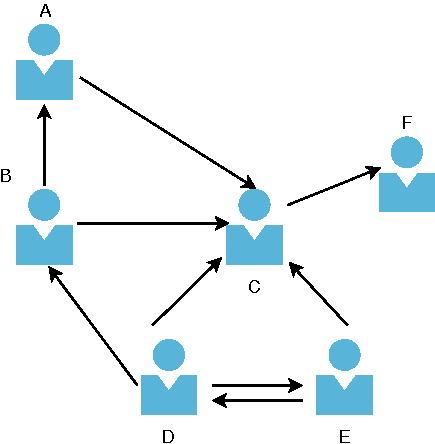
\includegraphics{capitulo_modelo/seguir_seguido.pdf} 
  \caption{As relações de seguir e poder ser seguido no GitHub. Adaptado de \cite{mo2015geminer}.}
  \label{fig:cap_modelo_seguir_seguido} 
\end{figure}

A equação \ref{eq:cap_modelo_equacao1_geminer} é a base do algoritmo PageRank. Como pode ser visto, trata-se de uma equação recursiva. Isso acontece pois para se calcular a relevância de um colaborador é necessário calcular a relevância de todos os colaboradores que o seguem. 

A primeira parte da equação inicializa o \textit{pagerank} de cada elemento ao dividir o número 1 - $d$ pela quantidade de colaboradores em todo o grafo sendo analisado. Sendo que $d$ é o chamado \textit{dumping factor} e indica a probabilidade de que no próximo passo o algoritmo calcule a relevância de um nó adjacente ao atual ou de um nó qualquer aleatório do grafo.  O valor sugerido para  $d$  pelos autores é de 0.85. Os vértices do grafo analisado são representados pelas letras $u$ e $v$. Sendo assim, a equação representa o cálculo da relevância do vértice $v$ e, para isso, realiza uma soma da relevância de todos os outros vértices $u$ de tal forma que $u$ seja $v$. O elemento  $L(u)$ indica quantos outros colaboradores o colaborador $u$ também segue. 

\begin{equation}
\label{eq:cap_modelo_equacao1_geminer}
PR(v) =  \frac{1-d}{\mid V \mid} + d *  \sum_{(u,v) \in E}  \frac{PR(u)}{L(u)}
\end{equation}

Além de considerar o relacionamento ``seguir'' e ``ser seguido'', os autores consideram outros aspectos para avaliar a expertise de um colaborador. Eles nomeiam essa abordagem de \textit{Multi-Source PageRank} já que a classificação é realizada por meio de múltiplos atributos.   O outro aspecto utilizado para avaliar a expertise de um colaborador é o nível de popularidade dos projetos que ele contribuiu. Isso é feito de duas formas, a primeira é analisando quais colaboradores estão observando(\textit{watching}) o projeto. Quanto mais colaboradores relevantes observam um determinado projeto, maior é a relevância dele. A segunda forma de avaliar a relevância de um projeto é feita medindo a relevância dos colaboradores que contribuíram com o projeto.  Essas duas avaliações são realizadas por meio das equações \ref{eq:cap_modelo_equacao_watch_geminer} e \ref{eq:cap_modelo_equacao_contribuicao_projeto_geminer}  respectivamente. Na equação \ref{eq:cap_modelo_equacao_watch_geminer}, o conjunto $E_W$ representa as relações de observar entre colaboradores e projetos. Logo, nessa equação, são somados os \textit{pageranks} de todos os colaboradores $u$ que  observam o projeto $r$. Além disso, $L_W(u)$ representa a quantidade de projetos que o colaborador $u$ observa. Lembrando que essa divisão por  $L_W(u)$ é realizada para que um colaborador que observa muitos projetos não afete incorretamente o resultado final.  Na equação \ref{eq:cap_modelo_equacao_contribuicao_projeto_geminer} o conjunto $r(U)$ representa todos os colaboradores que contribuíram com o projeto $r$. Além disso, $L_C(u)$ representa a quantidade de projetos em que o colaborador $u$ já contribuiu.








\begin{equation}
\label{eq:cap_modelo_equacao_watch_geminer}
PR(r) =    \sum_{(u,r) \in E_W}  \frac{PR(u)}{L_W(u)}
\end{equation}

\begin{equation}
\label{eq:cap_modelo_equacao_contribuicao_projeto_geminer}
PR(r) = PR(r) +    \sum_{u  \in r(U) }  \frac{PR(u)}{L_C(u)}
\end{equation}

 Além dos já apresentados, os autores acrescentam mais dois atributos para calcular o \textit{pagerank} de um colaborador: o \textit{pagerank} dos colaboradores no qual ele já trabalhou em conjunto e o \textit{pagerank} dos projetos no qual o colaborador trabalhou. Os autores defendem que, de acordo com suas observações, colaboradores que contribuem frequentemente em projetos com outros colaboradores relevantes, provavelmente sejam também relevantes. Além disso, colaboradores que contribuem frequentemente em projetos relevantes, também provavelmente sejam relevantes para a comunidade.  Para incluir esses dois aspectos no cálculo do \textit{pagerank} dos colaboradores foram utilizadas as equações \ref{eq:cap_modelo_equacao_colaboracao_geminer} e \ref{eq:cap_modelo_equacao_pagerank_projeto_geminer}. Na equação  \ref{eq:cap_modelo_equacao_colaboracao_geminer}, o grupo$ E_C$ contém os pares de colaboradores que já  contribuíram no mesmo projeto. O número $L_C(u_22)$  é igual à quantidade de projetos em que o colaborador $u_2$ contribuiu. Os grupos $u1(R)$ e $us(R)$ representam, respectivamente, todos os projetos em que o colaborador $u_1$ contribuiu e  todos os projetos em que o colaborador $u_2$ contribuiu. Logo, a equação \ref{eq:cap_modelo_equacao_colaboracao_geminer}  é utilizada para adicionar ao \textit{pagerank} do colaborador $u_1$ o \textit{pagerank} de todos os colaboradores no qual o colaborador $u_1$ tenha atuado em conjunto no mesmo projeto. Já na equação \ref{eq:cap_modelo_equacao_pagerank_projeto_geminer}, o \textit{pagerank} do colaborador $u$ é somado ao \textit{pagerank} de todos os projetos no qual o colaborador $u$ tenha atuado.
 


\begin{equation}
\label{eq:cap_modelo_equacao_colaboracao_geminer}
PR(u_1) =  PR(u_1) +   \sum_{(u_1,u_2) \in E_C}  PR(u_2) * \frac{\mid u_1(R) \cap u_2(R)\mid}{L_C(u_2)}
\end{equation}

\begin{equation}
\label{eq:cap_modelo_equacao_pagerank_projeto_geminer}
PR(u) = PR(u) +    \sum_{r  \in u(R) }  \frac{PR(r)}{L_C(r)}
\end{equation}



Após a aplicação de todas essas fórmulas matemáticas, é calculado o \textit{pagerank} de cada colaborador. Quanto maior o \textit{pagerank}, maior o nível de relevância do colaborador dentro da comunidade de desenvolvimento de software. Porém, conforme dito anteriormente, isso não garante que colaboradores com um alto \textit{pagerank} sejam necessariamente especialistas em alguma tecnologia. Além disso, é preciso avaliar o volume de contribuição real que um colaborador realizou. No GEMiner isso é realizado observando a quantidade de linhas de código alteradas ou adicionadas pelo colaborador. Porém, em nossa pesquisa, utilizaremos uma medida alternativa. Em vez da quantidade de linhas de linhas de código alteradas, utilizaremos a quantidade média diária de \textit{commits} que cada colaborador realizou. A essa medida demos o nome de assiduidade. Essa pequena alteração em relação à abordagem original do GEMiner foi realizada devido à dificuldade de calcular a quantidade de linhas alteradas ou modificadas em um conjunto grande de projetos. Mais detalhes a respeito dessa alteração e de como implementamos o GEMiner serão fornecidos no estudo de caso apresentado no Capítulo \ref{cap_estudo_caso}.

\subsubsection{Assiduidade dos colaboradores}

Para medir a assiduidade de um colaborador vamos calcular qual a média diária de contribuições e compará-la com a média geral de todos os colaboradores. Essas contribuições serão calculadas por meio de uma contagem dos \textit{commits} que esse colaborador realizou.  De acordo com Loeliger et al \cite{loeliger2012version}, um \textit{commit} é uma alteração nos arquivos de um projeto. Essa alteração pode ser composta pela inclusão e remoção de dados ou arquivos. Além disso, um \textit{commit} contém informações a respeito do seu autor. Isso permite rastrear o histórico de um projeto e identificar quem foi responsável por cada uma das mudanças.  Utilizaremos a frequência média de \textit{commits} que um colaborador realiza em um projeto como base para estimar a assiduidade de um colaborador em relação a um projeto. A assiduidade de um colaborador será calculada pela distância entre a sua média de \textit{commits} e a média geral de todos os colaboradores daquele projeto.



\subsubsection{Índice de colaboração}

O índice de colaboração($I_c(r)$) será o valor numérico final a ser utilizado como entrada para o modelo de análise de produtividade dos projetos.  Esse índice será calculado para cada projeto $r$ de acordo com a equação \ref{eq:cap_calculo_indice_colaboracao}. A função $A(u)$ representa a assiduidade do colaborador $u$ enquanto a função $Q(u)$ representa a qualidade do colaborador $u$. O conjunto $u(R)$ representa todos os colaboradores que realizaram alguma contribuição no projeto $r$.


\begin{equation}
\label{eq:cap_calculo_indice_colaboracao}
I_c(r) =  \sum_{u  \in u(R) } A(u) * Q(u)
\end{equation}

\section{Saídas}
\label{secao_modelo_concreto_saidas}

Conforme descrito na seção \ref{modelo_concreto_saidas} existe uma restrição quanto à escolha das saídas que serão utilizadas no modelo de produtividade: elas precisam estar estatisticamente correlacionadas com as entradas. A única forma de garantir isso, é verificando a significância dessa correlação. Essa verificação só pode ser realizada se utilizando os dados reais dos projetos que serão analisados. Com isso, a definição definitiva das saídas não pode ser feita antes que os dados tenham sido obtidos. Entretanto, listaremos algumas das métricas candidatas a serem utilizadas. Essas métricas foram escolhidas por intuitivamente terem relação com as entradas. Porém, essa relação só será devidamente verificada no estudo de caso realizado no Capítulo \ref{cap_estudo_caso}. 

\subsection{Linhas de código}


A primeira saída a ser utilizada no modelo de produtividade será a quantidade de linhas de código. Essa métrica é uma das mais utilizadas, tanto no âmbito teórico quanto no prático, para representar o tamanho do software.  No contexto da pesquisa em engenharia de software, ela tem sido utilizada extensivamente como uma preditora do esforço que foi ou será gasto para a criação do software.  Essa métrica foi uma das escolhidas para representar o tamanho no contexto dos softwares livres por algumas razões. A primeira delas é o aspecto prático: ela pode ser calculada utilizando métodos automáticos de contagem. Essa característica é especialmente relevante no contexto desta pesquisa já que iremos analisar uma grande quantidade de projetos. Uma métrica que exigisse algum tipo de intervenção manual seria naturalmente inviável. Esse seria o caso se usássemos uma métrica como os pontos por função. Não teríamos como medi-la automaticamente. Ao invés disso, teríamos de usar alguma abordagem qualitativa e isso inviabilizaria a análise de uma grande quantidade de projetos. 

Como pode imaginar-se, a contagem de linhas de código é uma métrica longe de ser perfeita para avaliar o tamanho do sofware. Bahtt et al. \cite{bhatt2012analysis} descreve algumas das desvantagens dessa métrica:

\begin{itemize}
\item Elas não conseguem captar plenamente o esforço realizado pelos desenvolvimento. De acordo com Hoffman\cite{hoffman2000darker}, apenas por volta de 35\% do esforço realizado pelos desenvolvedores é convertido diretamente em linhas de código.
\item Elas não estão necessariamente relacionadas com as funcionalidades oferecidas pelo software. Por exemplo, muito código pode ser desenvolvido para a realização de apenas uma funcionalidade. Logo, esse comportamento pode influenciar negativamente a utilização das linhas de código em uma avaliação de produtividade.
\item Entre os desenvolvedores podem existir costumes sintáticos distintos fazendo com que haja uma divergência na quantidade de linhas de código utilizadas para escrever uma mesma parte do software. Algumas dessas divergências podem ser amenizadas pela estratégia utilizada para contar as linhas de código. Podem ser realizadas alterações no código original antes de contar a quantidade de linhas. Essas alterações obviamente não devem alterar a lógica do programa, mas podem servir para remover essas diferenças sintáticas que prejudiquem a contagem. Ainda assim, boa parte da literatura indica que a quantidade de linhas de código nunca deve ser  a única métrica utilizada para avaliar a produtividade individual de algum desenvolvedor.
\end{itemize}

Apesar dos problemas apresentados em utilizar as linhas de código como uma métrica de tamanho, também podemos encontrar na literatura pesquisas que utilizaram essa métrica de forma bem sucedida\cite{maccormack2003trade,funk2005application,sudhakar2012measuring,tan2009productivity}. Analisando essas pesquisa, podemos encontrar a indicação de cuidados importantes que devem ser considerados ao utilizar as linhas de código como uma métrica de tamanho:

\begin{itemize}
\item Essa métrica não deve ser utilizada para comparar linguagens diferentes. \cite{rosenberg1997some,park1992software}.
\item Não existe uma padronização amplamente aceita sobre como essa métrica deve ser calculada. Apesar da existência de esforços como o padrão criado pelo instituto de software da universidade Carnegie-Mellon\cite{park1992software}. Essa falta de um padrão definitivo acontece pelas diferenças significativas entre as linguagens de programação existentes e o fato de que novas linguagens, com sintaxes diferentes, são criadas constantemente.
\end{itemize} 


Uma outra alternativa seria medir o tamanho do software utilizando a quantidade de arquivos. Inclusive realizaremos a medição desse dado durante o nosso estudo de caso. Porém, estudos recentes mostram que não há diferenças significativas entre essas duas medidas. Um exemplo é a pesquisa realizada por Herraiz et al.\cite{herraiz2006comparison}. Nelas os autores mostram, por meio da análise empírica de projetos de software livre, que o padrão de crescimento desses projetos é o mesmo, independente da métrica utilizada. Ou seja, medindo o tamanho dos projetos em linhas de código ou número de arquivo leva a resultados muito semelhantes. Por isso, elencaremos apenas a quantidade de linhas de código em vez de utilizarmos uma agregação das duas medidas.



\subsection{\textit{Pull Requests}}

A base para a filosofia de software livre é a contribuição voluntária. Essa contribuição, no contexto dos software livre, tem sido realizada com o auxílio de repositórios de software como o GitHub, BitBucket, GitLab, SourceForge, e Lauchpad. Esses repositórios normalmente utilizam um modelo de controle de versão distribuído. Nesse modelo, o software não fica armazenado em um único e exclusivo repositório central. Ao invés disso, cada colaborador possui uma versão dos arquivos para o controle de versão. Esses arquivos locais podem, inclusive, ser a base para um novo repositório que evolua o projeto de uma forma diferente da realizada no repositório original. Porém, para inserir, no repositório original, as mudanças realizadas em um repositório paralelo, é utilizado um recurso chamado de \textit{pull request}. Nesse modelo as mudanças são primeiro avaliadas antes de serem incluídas definitivamente no projeto. Essa avaliação pode consistir na verificação automática de conformidade do novo código com regras previamente definidas como também a execução automática de testes de software. Além disso, dentro de um \textit{pull request}, normalmente é possível discutir essas mudanças. Essa discussão pode envolver uma avaliação funcional que verifique a efetiva necessidade de a mudança ser feita como também pode envolver discussões técnicas como o impacto da mudança no desenho e arquitetura do software.  Ao final dessa discussão, a mudança pode ser aprovada ou rejeitada.  Quanto mais \textit{pull request} um projeto tem, maior o nível de interesse da comunidade em contribuir com o projeto. Acreditamos que com isso o projeto está atingindo um dos objetivos do software livre: maior interesse da comunidade em colaborar. Ou seja, elencamos a quantidade de \textit{pull requests} como uma possível medida de saída pelo qual faz sentido considerar a constância em que colaboradores externos conseguem contribuir para um projeto como um aspecto da evolução do projeto. Quanto mais pessoas interessadas em contribuir, maior o projeto.

\subsection{Popularidade}


Conforme expresso anteriormente, há o que se questionar na relação entre a quantidade de linhas de código de um software e o número de funcionalidades que ele disponibiliza para seus usuários e outros interessados. Pode haver uma diferença significativa entre esses dois aspectos. Logo, faz sentido incluir em nosso modelo de avaliação de produtividade, alguma métrica que seja utilizada na tentativa de capturar a quantidade ou valor das funcionalidades que um software fornece aos seus usuários. Por isso, para nosso modelo específico, inserimos a popularidade do projeto como uma possível métrica de saída para o modelo de estimação de produtividade. Essa popularidade será avaliada utilizando as funcionalidades presentes no repositório de software sendo utilizado. No caso do GiiHub, que é o repositório que utilizaremos no nosso estudo de caso do Capítulo \ref{cap_estudo_caso}, são fornecidas duas ferramentas para que um usuário possa indicar seus interesses ou sua aprovação em relação a um projeto: estrelas e \textit{watch}. Ao dar uma estrela para um projeto o usuário indica que acha aquele projeto  relevante e que gostaria, de alguma forma, marcá-lo para tê-lo associado a sua conta. Todos os projetos marcados com estrelas podem ser consultados em uma página da conta do usuário.  Ao dar um \textit{watch} em um projeto, o usuário irá receber notificações a respeito do projeto. Essas notificações incluem dentre outras, a liberação de uma nova release, a criação de \textit{issues} e seus comentários e a criação de \textit{pull requests}.


\section{Método de agrupamento dos projetos semelhantes}

No modelo concreto de estimação dos juros da dívida técnica em projetos de software livre utilizamos o LDA(\textit{Latent Dirichlet Allocation}) para agrupar os projetos semelhantes. Utilizaremos essa técnica por dois motivos. O primeiro é o fato de que grande parte dos software livres possuem algum documento que descreve as suas funcionalidades. Esse documento pode ser usado pelo LDA para estimar qual o assunto do texto e consequentemente à qual domínio o software pertence. O segundo motivo é a existência de experimentos na literatura que utilizaram o LDA de forma satisfatória para a categorização de projetos de software livre. Um exemplo que foi utilizado como uma das bases para a implementação realizada no Capítulo \ref{cap_estudo_caso}  é o trabalho de Ray. et al. \cite{ray2014large}. Nessa pesquisa os autores realizam uma extensa mineração de dados para analisar as relações entre as linguagens de programação e o número de defeitos nos projetos de software livre. Assim como nesta pesquisa, os autores tiveram a necessidade de apenas comparar projetos que fossem de um mesmo domínio de aplicação já que o domínio poderia influenciar o número de defeitos dos projetos. Por isso, eles aplicaram o LDA para categorizar os projetos de acordo com o domínio de aplicação e, assim, eliminar essa possibilidade de interferência nos resultados.

\section{Método de particionamento dos grupos de projetos}

Conforme assinalado anteriormente, só podemos definir qual o limiar entre um projeto considerado de produtividade ótima ou produtividade afetada, após termos obtidos os dados dos projetos.  Essa etapa de definição do método de particionamento dos grupos para o modelo concreto será realizada apenas no estudo de caso do capítulo  Capítulo \ref{cap_estudo_caso}.


\section{Conclusões}
Neste capítulo propusemos um modelo para a estimação dos juros da dívida técnica em projetos de desenvolvimento de software. Esses modelos são baseados no conceito de que os juros são a diminuição causada pela existência da dívida técnica, da produtividade. Além do modelo mais abstrato, foram fornecidos detalhes de quais definições são necessárias para que esse modelo possa ser aplicado. Por fim, descrevemos a aplicação do modelo abstrato para estimação dos juros em projetos de software livre.





 
 
 